\documentclass[14pt]{extarticle}

\let\Overrightarrow\overrightarrow
\let\vecarrow\overrightarrow


%other%
\usepackage{graphicx}
\usepackage{float}
\usepackage[margin=0.7in]{geometry}
\usepackage{caption}
\usepackage{csquotes}
\usepackage[export]{adjustbox}
\usepackage{wrapfig}
\usepackage{setspace}
\usepackage{anyfontsize}
\usepackage{titlesec}
\titleformat{\section}{
	\normalfont\fontsize{20}{20}\bfseries}{\thesection}{1em}{}
\titleformat{\subsection}{
	\normalfont\fontsize{17}{20}\bfseries}{\thesubsection}{0.1em}{}
\usepackage{relsize}
%other%



%%\newcommand{\F}{\Oldmathbfcal{F}}
%math%
\usepackage{amsthm}
\usepackage{amssymb}
\usepackage{amsmath}
\usepackage{mathtools}
%%\usepackage[cal = pxtx, scr = dutchcal]{mathalfa}



%\usepackage{unicode-math}
%\newtheorem*{}{\textup{Лемма}}
\newtheorem*{theorem}{\textup{Теорема}}
\newtheorem*{remark}{\textup{Комментарий}}
%\renewcommand\qedsymbol{$\blacksquare$}
%\usepackage{parskip}

\usepackage{pgfplots}
\usepgfplotslibrary{polar}
\usepgflibrary{shapes.geometric}
\usetikzlibrary{calc}


\renewenvironment{proof}
    {\noindent \textit{Доказательство.}\\
	\indent $\square$}
	{ $\blacksquare$\\ }

\newenvironment{solution}
	{\vspace{-4.3mm} \noindent\textbf{Решение.}}


\renewenvironment{remark}
    {\noindent\textbf{Коментарий}}

\usepackage{tikz}
   \usetikzlibrary{calc}

\newcommand{\arc}[0]{
   \tikz [baseline = (N.base), every node/.style={}] {
	  \node [inner sep = 0pt] (N){}; %{$#0$};
      \draw [line width = 0.8pt] plot [smooth, tension=1.3] coordinates {
         ($(N.north west) + (-1.5ex,0.6ex+0.4ex)$)
         ($(N.north)      + (-0.75ex,0+0.4ex)$)
         ($(N.north east) + (0ex,0.6ex+0.4ex)$)
      };
   }
}

\renewenvironment{rcases}
  {\left.\begin{aligned}}
  {\end{aligned}\right\rbrace}

\DeclarePairedDelimiter\abs{\lvert}{\rvert}
\DeclarePairedDelimiter\norm{\lVert}{\rVert}

%\newcounter{example}[section]
\newenvironment{example}[1]{\noindent \textbf{Пример #1.}}

\let\mathb\mathbb


\newcommand{\N}{\mathb{N}}
\newcommand{\Z}{\mathb{Z}}
\newcommand{\R}{\mathb{R}}
\newcommand{\F}{\mathbfcal{F}}
\renewcommand{\P}{\mathbfcal{P}}
%\newcommand*{\Z}{\mathbb{Z}}
%math%

%fonts%
\usepackage[russian]{babel}
\usepackage{polyglossia}
\setdefaultlanguage[spelling=modern]{russian}
%\setotherlanguage{english}
\setmainfont{CMU Serif}
\setsansfont{CMU Sans Serif}
\setmonofont{CMU Typewriter Text}  
%\setmathfont{Latin Modern Math}
\usepackage{mathrsfs}
%\DeclareMathAlphabet{\mathcal}{T1}{TX}{m}{n}

\usepackage{unicode-math}


%\let\Oldmathbfcal=\mathbfcal
%\renewcommand{\mathbfcal}{\mumble\Oldmathbfcal}

%%\newcommand{\F}{\Oldmathbfcal{F}}
%%\newcommand{\F}{𝓕}

%\usepackage{fontspec}
\setmathfont{Latin Modern Math}

\DeclareSymbolFont{symbols}{OMS}{cmsy}{m}{n}
\DeclareSymbolFont{bsymbols}{OMS}{cmsy}{b}{n}
\DeclareSymbolFontAlphabet{\mathcal}{symbols}
\DeclareSymbolFontAlphabet{\mathbfcal}{bsymbols}

%\setmathfont[range = {2131}]{AMS}
%\usepackage{amsfonts}
%\usepackage{dsfont}
%fonts%


\begin{document}

\begin{figure}[H]
    \centering
    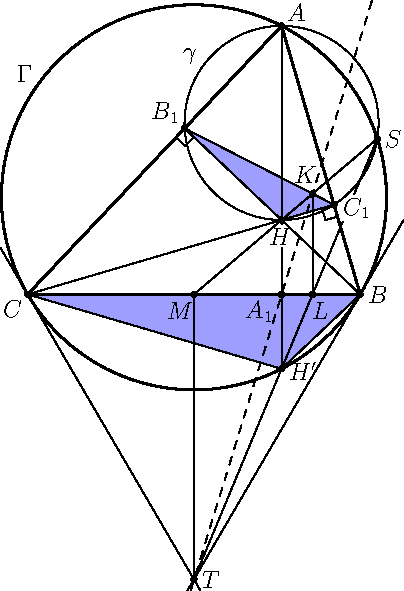
\includegraphics[height=15cm]{fig.pdf}
\end{figure}


Пусть \(\Gamma\) -- окружность, описанная около треугольника \(ABC\); 
\(A_1\), \(B_1\), \(C_1\) -- основания высот из соответствующих вершин; 
\(\gamma\) -- окружность, описанная около треугольника \(AB_1C_1\);
\(M\) -- середина \(BC\). Пусть точка \(H'\) симметрична \(H\) относительно 
\(BC\) (очевидно, что \(H' \in \Gamma\)). Пусть также \(T\) -- точка 
пересечения касательных к \(\Gamma\), восстановленных в точках \(B\) и 
\(C\), \(K = MH \cap B_1C_1\), \(L = TH' \cap BC\), а \(S\) 
-- вторая точка пересечения \(\Gamma\) с \(\gamma\) 
(отличная от \(A\)). Наша цель доказать, что 
точки \(K\), \(A_1\), \(T\) --- коллинеарны (лежат на одной прямой)

Как известно, \(S\) -- центр поворотной гомотетии \(\F\), переводящей 
\(B_1C_1\) в \(CB\). При этом \(\F(\gamma) \rightarrow \Gamma\). 
Покажем, что \(\F(H) \rightarrow H'\). 
Сразу отметим, что \(M\) -- точка пересечения касательных к \(\gamma\), 
восстановленных в точках \(B_1\) и \(C_1\) (доказывается простым счётом 
углов). Таким образом \(\F(M) \rightarrow T\). Поскольку 
\(\angle C_1B_1H = \angle BCH = \angle BCH'\), то с учётом 
вышесказанного получаем, что действительно \(\F(H) 
\rightarrow H'\). А отсюда следует, что \(\F(K) = L\).

Теперь воспользуемся тем, что \(\F(H) \rightarrow H'\) и 
\(\F(M) \rightarrow T\). А тогда, в силу свойств поворотной 
гомотетии, точка \(S\) также является поворотной гомотетией 
\(\P\), переводящей \(HH'\) в \(MT\). Теперь заметим, что 
\(MT \perp CB \perp HH'\) \(\Rightarrow MT \parallel HH'\), 
а значит \(\P\) на самом деле гомотетия (с центром \(S\)). 
Откуда получаем, что \(M, H, K, S\) коллинеарны и 
\(T, H', L, S\) коллинеарны. Вернёмся к \(\F\). Так как 
\(\F(H) \rightarrow H'\) и \(\F(K) \rightarrow L\), то 
\(\dfrac{HK}{H'L} = \dfrac{SK}{SL}\), откуда \(LK \parallel 
HH'\) по теореме Фалеса.

Теперь осталось записать несколько подобий треугольников, 
воспользовавшись найденными паралельностями.\\
1) \(\triangle MHA_1 \sim \triangle MKL\) (гомотетичны с 
центром в \(M\))\\
\indent \(\dfrac{A_1H}{KL} = \dfrac{MA_1}{ML}\)\\

\noindent 2) \(\triangle LA_1H' \sim \triangle LMT\) 
(гомотетичны с центром в \(L\))\\
\indent \(\dfrac{A_1H'}{MT} = \dfrac{LA_1}{ML}\)\\

\noindent Отсюда получаем, что \(\dfrac{MT}{KL} = 
\dfrac{MA_1}{LA_1}\) (так как \(A_1H = A_1H'\)). 
Теперь остаётся лишь заметить, что прямоугольные треугольники 
\(LA_1K\) и \(MA_1T\) подобны ввиду последнего соотношения, 
а это равносильно коллинеарности точек \(T, A_1, K\).

\end{document}
